% ------------------------------------------------------------------------
% Name: Introduction
% Author: Emmanuel SCHWARTZ
% Date: November 2016
% Description: Introduction Chapter for my master thesis paper
% ------------------------------------------------------------------------

\section{Motivation}
\paragraph{}
It is often considered that the history of electronic mail (or e-mail) begins in 1965, at a time when the Internet did not even exist yet. By that time, the first exchanges of messages was only possible between users on private networks were set up. One of the first systems to allow message exchange was the Competent Time-Sharing System (CTSS) of the famous Massachusetts Institute of Technology (MIT), although this paternity has also been claimed by System Development Corporation SDC) and its own Time-Sharing System created for the Q32, a computer specially manufactured by IBM for the US Air Force.
\paragraph{}
However, e-mail is only really born from the creation of the ARPAnet network, the ancestor of the Internet. In 1971, after writing some 200 lines of code in order to create two applications, SNDMSG nas READMAIL, the engineer named Raymond Samuel Tomlinson could sent the first email of history to himself. Some times later, 
Tomlinson found a way for the program to easily differentiate a local message from a network message: the symbol @ was born. It was a simple way to ​​dissociate a user name and host name with the only character that was not used in any proper name nor, above all, in any company name. The first "netmail" test was sent with only content "QWERTYUIOP", the first line of character of the English keyboard.
\paragraph{}
The email was so successful that it quickly became unthinkable for users of the ARPAnet network to do without it. As a result, the software quickly became the "killer app"  of the ARPAnet network, and developers focused either on improving the program and its transfer protocol, or creating their own solutions. In 1992, a great improvment was made: the world's first-ever email attachment, sent by the researcher Nathaniel Borenstein, where we could see a adorable photo of his barbershop quartet, The Telephone Chords. This was made possible thanks to MIME (Multipurpose Internet Mail Extensions),a internet standard that extends the data format of e-mails.
\paragraph{}
Fourty years later, despite the creation of Instant Messaging, or some years later, social networks, e-mails are still very popular: 183 billion of them are sent every day! If e-mails spam remains a major problem, e-mails has to face new challenges: \textbf{Reliability} \& \textbf{Privacy}. 
\paragraph{}
When a person is sending an e-mail, she expects that her message will be received successfully by the
intended recipient. For most cases, it does, but sometimes, for the following reasons, it does not:
\begin{easylist}[enumerate]
\ListProperties(Hide=100, Hang=false, Progressive=3ex, Style*=--)
& The design of e-mail: Two users does not have to be online at the same time in order to communicate. This is called asynchronious communications. This is made possible by the mail servers, accepting messages from sources and attempt to relay them towards, or deliver them to, the recipient. In order to do so, e-mails have to jump from an server to an other: Some e-mails might get lost during these operations, for various reasons (busy servers, e-mails deferral, rejected e-mails)
& The exponential groth of e-mail spam has forced the use of e-mail rejection, intended to identify and separate legitimate e-mails from junk e-mails. Unfortunately, this has turned out into a false positive problem: Some legimate e-mails are considered as junk, this means the user thinks he did not receive the e-mail.
Some solutions try to solve these problems such as RE: Reliable Email[*], which tries to create an intelligent filter for e-mails, or tools that responds automatically to undeliverability by persisting with retransmission or retransmitting to alternate recipients [*]
\end{easylist}
\paragraph{}
Alongside with \textbf{reliability}, e-mail is facing one of the biggest challenges: \textbf{Privacy}. Since the shattering revelations of Edward Snowden, brigging to light the massive world surveillance by the U.S, people try to protect themselves by encypting their communications when possible. The famous free email application, Mozilla Thunderbird has an extension called EnigMail, which can encrypt e-mails thanks to OpenPGP. The downside is, that every user needs to have this add-ons installed, otherwise it will be not possible to read the e-mail that was intented for him. A solution could be that Thunderbird integrates directly this feature in his client, but is still not planned on the road map.
But a recent piece of news[*] unviels that the IT-idustry giants such as Google, Microsoft, Yahoo!, LinkedIn and Comcast are working together to elaborate a new encrypted messaging protocol, named SMTP STS (Strict Transport Security)[*]. The idea is that a session starts in clear, and after the server announces that it supports the encrypted connection, the client can then switch to encryption mode, to avoid man-in-the-middle attack. Unfornately no released date was announced yet. 
\paragraph{}
Last downside of e-mails involves the user. Nowadays, it is common practice to send business documents via e-mail or via supplier\textquoteright s web portal: Faster and cheaper compared to a hard copy sent via post. But, how can a user successuffly order and sort out differents kinds of documents, coming from different mailboxes? In most cases, the user does not have a clue how to establish a \textbf{document management}: local storage? cloud storage? And what if the computer has hard drive failures, or is infected by viruses: Did they make regular back-ups?
\paragraph{}
With respect to the application senario described in the next section, this thesis will try to answer these problems with new upcoming technologies such as blockchains, decentralized storage and Dapps. 
 
\section {Application Scenario}
\paragraph{}
 Even if the big actors of Internet are trying to adapt e-mails to nowadays requirements, e-mails might not be the right solution anymore to send buisiness documents. Figure 1.1 shows the path that an e-mail takes to go from the company to a client, jumping through servers via the protocol SMTP. Once the email has eached the client's mail server, the client has the choice to synchronize his email between 3 protocols: IMAP, POP3 or SMTP.
\begin{figure}[htp]
\centering
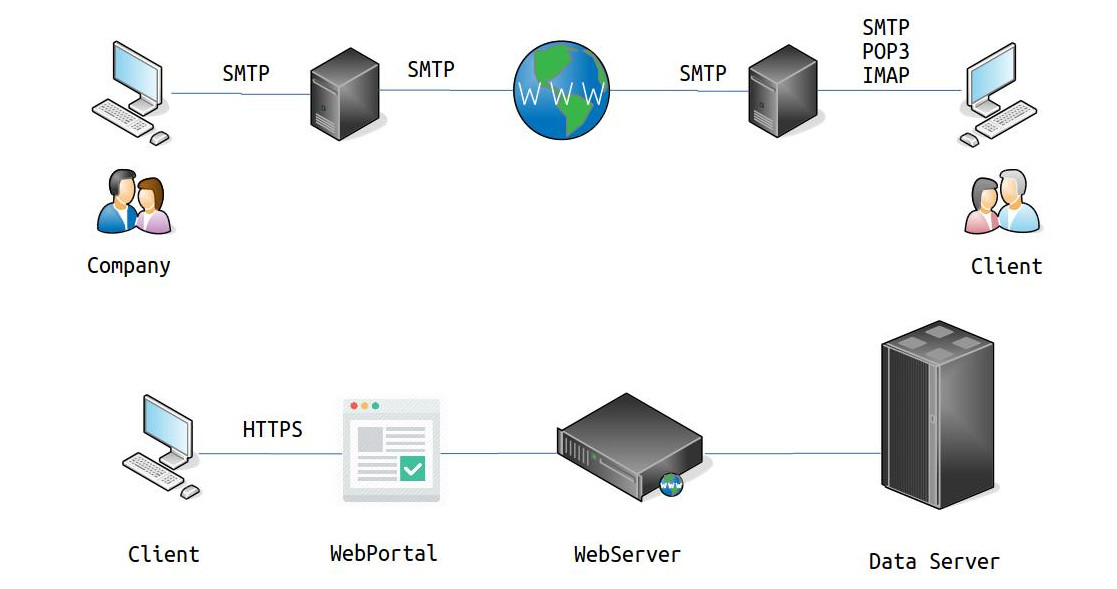
\includegraphics[scale=0.49]{/home/emmanuel/Documents/master-thesis/doc/ressources/email&webportal.jpg}
\caption{}
\label{}
\end{figure}
\newline
New technologies that Bitcoin has brought, paired up with decentralized storage providers, can revolutionize the way we are going to send documents, described in the figure 1.2. 
\begin{figure}[htp]
\centering
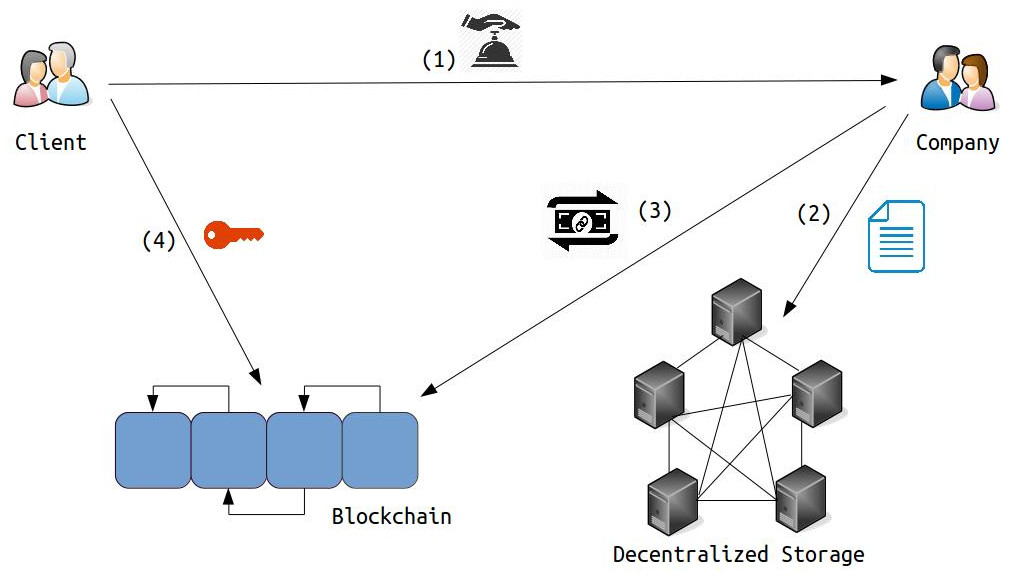
\includegraphics[scale=0.47]{/home/emmanuel/Documents/master-thesis/doc/ressources/blockchain.jpg}
\caption{}
\label{}
\end{figure}
\newline
The customer is creating a request to the company for a specific document (1). Then, the document is stored using a distributed storage provider (2). A link is created, which is stored directly in the blockchain by doing an transaction (3). The blockchain transaction provides the evidence, that the document has been sent and keeps a permanent not alterable link to the document. In order to open a document, the customer only needs its private key (4). (For further explanation, see 2.2)

\section{Objective}
\paragraph{}
The main goal of this thesis is to see if there is a possible implementation of a proof of concept (poc) using the new technologies such as blockchains, decentralized storage and Dapps to send documents between a company and a customer. Pros and Cons will be also discussed. Additionnally, MetaData can give useful information such as the author of a document, the timestamp, some comments etc etc. This thesis will show if metadata can be added during a transaction. Besides these constraints, a document should be also signed Within the proposed architecture. Furthermore, a flexible approach is desirable that supports multiple storage providers such as Amazon, Azure, IPFS, StorJ. Last but not least, this implemantation should be able to be combined with traditional cloud systems.
\newline
In summary, the objective is to find a proof of concept that can send documents between two users with the following points:
\begin{easylist}[enumerate]
\ListProperties(Hide=100, Hang=false, Progressive=3ex, Style*=--)
& A dvantages and limitations of this architecture
& Signing a document with this architecture?
& Combination with traditional cloud systems
& Flexible regarding storage providers
& Easy \& intuitive GUI for users
& Metadata
\end{easylist}

\section{Overview}
\paragraph{}
\textbf{!!!!!!!!!!!!!!!!!!!!!!!! TBD !!!!!!!!!!!!!!!!!!!}
To achieve the objectives stated in section 1.3, chapter 2 - Related Work and Basic Principles - contains an in-depth overview of state of the decentralized document management.
TDB: 2.1, 2.2, 2.3 etc
Chapter 3 presents the method.
Chapter 4: evaluate the proposed approaches  
Finally, chapter 5 concludes the work and highlights the applicability of the developed approaches to other domains. 
